%-------------------------------------------------------------------------------
% 请勿删除本注释
% Free Response Question 2
%
% 指引:
% 如在小问之前有通用问题描述,请放置于此
%-------------------------------------------------------------------------------
\begin{figure}[H]
\centering
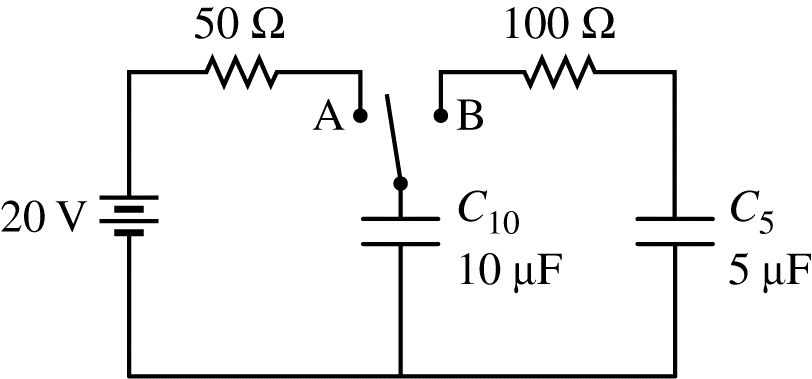
\includegraphics[scale=0.3]{images/img-020-032.png}
\end{figure}


\question
In the circuit above, the two capacitors are initially uncharged and the switch is initially open. At time $t=0$ the switch is moved to position A. % 请删除并替换本行,与上一行 \question 之间不要留空行

\begin{parts}

%-------------------------------------------------------------------------------
% 请勿删除本注释
% Part (a)
%
% 指引:
% 如在小问之前有通用问题描述,请放置于此
%-------------------------------------------------------------------------------

\part
Calculate the current in each of the two resistors immediately after the switch is moved to position A. % 请删除并替换本行,与上一行 \part 之间不要留空行
\begin{subparts}
\subpart Current in the $50 \Omega$ resistor
\subpart Current in the $100 \Omega$ resistor
\end{subparts}

%-------------------------------------------------------------------------------
% 请勿删除本注释
% Part (b)
%
% 指引:
% 如在小问之前有通用问题描述,请放置于此
%-------------------------------------------------------------------------------

\part
  % 请删除并替换本行,与上一行 \part 之间不要留空行
\begin{subparts}
\subpart Determine the amount of charge stored on the bottom plate of the $10 \mu \mathrm{F}$ capacitor a long time after the switch is moved to position $\mathrm{A}$.
\subpart Indicate the sign of the charge on the bottom plate of the $10 \mu \mathrm{F}$ capacitor.
\end{subparts}

\underline{\qquad}Positive \qquad   \underline{\qquad}Negative

%-------------------------------------------------------------------------------
% 请勿删除本注释
% Part (c)
%
% 指引:
% 如在小问之前有通用问题描述,请放置于此
%-------------------------------------------------------------------------------

Some time later, the switch is moved to position B.

\part
On the axes below, sketch a graph of the current $I$ in the $100 \Omega$ resistor as a function of time $t$ after the switch is moved to position B. Explicitly label any intercepts, asymptotes, maxima, or minima with numerical values or algebraic expressions, as appropriate. % 请删除并替换本行,与上一行 \part 之间不要留空行


\begin{figure}[H]
\centering
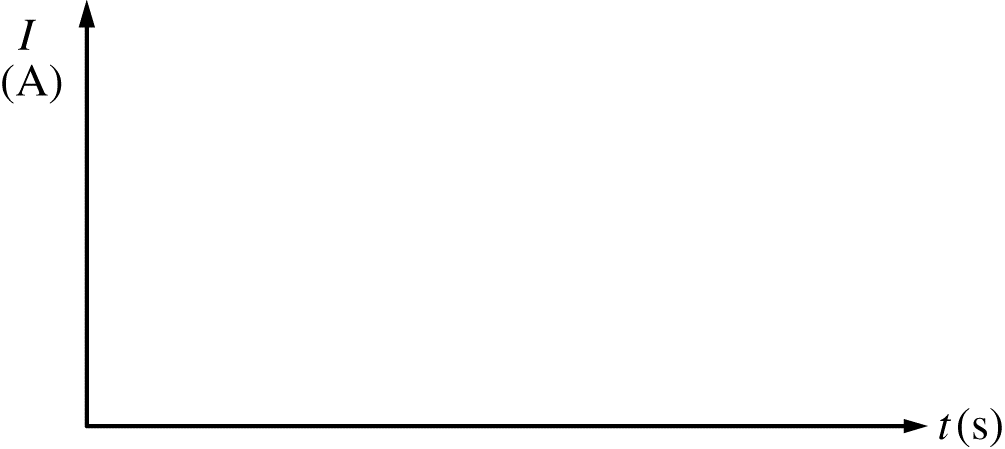
\includegraphics[scale=0.3]{images/img-021-033.png}
\end{figure}


%-------------------------------------------------------------------------------
% 请勿删除本注释
% Part (d)
%
% 指引:
% 如在小问之前有通用问题描述,请放置于此
%-------------------------------------------------------------------------------

\part
 Calculate the amount of charge on each capacitor a long time after the switch has been moved to position B.  % 请删除并替换本行,与上一行 \part 之间不要留空行

%-------------------------------------------------------------------------------
% 请勿删除本注释
% Part (e)
%
% 指引:
% 如在小问之前有通用问题描述,请放置于此
%-------------------------------------------------------------------------------

\part
Calculate the total energy dissipated in the $100 \Omega$ resistor after the switch is moved to position $\mathrm{B}$. % 请删除并替换本行,与上一行 \part 之间不要留空行

\end{parts}
